\textbf{Softwarové inženýrství} je inženýrská disciplína zabývající se praktickými problémy vývoje rozsáhlých softwarových systémů.

\subsection{Softwarový proces}
\textbf{Softwarový proces} je po částech uspořádaná množina kroků směřujících k vytvoření nebo úpravě softwarového díla.
\begin{itemize}
\item Krokem může být \textbf{aktivita} nebo opět \textbf{podproces} (hierarchická dekompozice procesu). 
\item Aktivity a podprocesy mohou \textbf{probíhat v čase souběžně}, tudíž je vyžadována jejich koordinace. 
\item Je \textbf{nutné zajistit opakovatelnost použití procesu ve vztahu k jednotlivým softwarovým projektům}, tedy zajistit jeho \textbf{znovupoužitelnost}.  Cílem je dosáhnout stabilních výsledků vysoké úrovně kvality.
\item Řada činností je zajišťována lidmi vybavenými určitými schopnostmi a znalostmi a majícím k dispozici technické prostředky nutné pro realizaci těchto činností.
\item \textbf{Softwarový produkt} je realizován v kontextu organizace s danými ekonomickými možnostmi a organizační strukturou.
\end{itemize}

\subsection{Modely softwarového procesu}
Vzhledem k tomu, že vývoj softwaru je relativně nová problematika dodnes není jasně definováno jak by měl správný softwarový proces vypadat. Byla však vyvinuta řada různých přístupu k vývoji softwaru. Lze říct, že základem všech je vodopádový model, který lze nalézt ve většině používaných přístupů.

\subsubsection{Vodopádový model}
Vychází z \textbf{rozdělení životního cyklu softwarového díla} na \textbf{čtyři} základní fáze:
\begin{enumerate}
\item \textbf{analýza požadavků} a jejich \textbf{specifikace},
\item \textbf{návrh} softwarového systému,
\item \textbf{implementace},
\item \textbf{testování} a udržování vytvořeného produktu.
\end{enumerate}
Princip vodopádu spočívá v tom, že \textbf{následující množina činností spjatá s danou fází} nemůže započít dříve, než skončí předchozí. Jinými slovy, výsledky předchozí fáze „vtékají“ jako vstupy do fáze následující.
\\\\
\noindent\makebox[\textwidth]{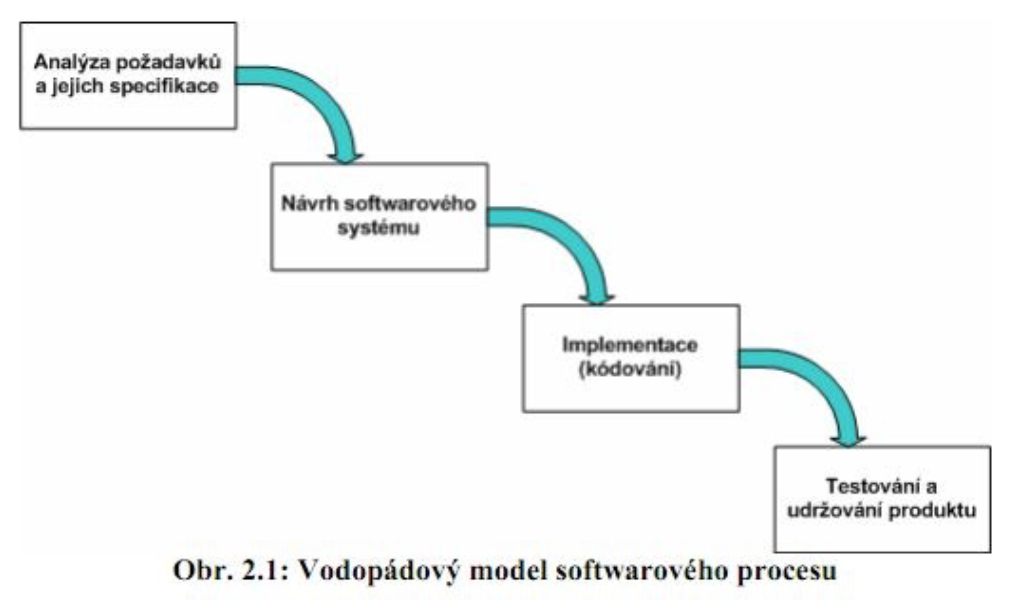
\includegraphics[width=12cm]{assets/swi1}}
Model je možno v \textbf{různých modifikacích} a \textbf{rozšířeních} nalézt ve většině současných přístupů. Tyto modifikace vznikly především kvůli odstranění některých jeho \textbf{nedostatků}, mezi které patří:
\begin{itemize}
\item \textbf{Prodleva} mezi zadáním projektu a vytvořením spustitelného systému je příliš dlouhá.
\item \textbf{Výsledek závisí} na \textbf{úplném a korektním zadaní požadavků} kladených na výsledný produkt.
\item \textbf{Nelze odhalit výslednou kvalitu produktu} danou splněním všech požadavků, dokud není výsledný softwarový systém hotov.
\end{itemize}

\subsubsection{Modifikace Vodopádového modelu}
\begin{itemize}
\item \textbf{Inkrementální} -- \textbf{postupné vytváření verzí} softwaru zahrnující postupně širší spektrum funkcí definovaných v průběhu jeho vytváření. V podstatě se jedná o \textbf{více menších vodopádů provedených za sebou} tak, aby každý z nich odpovídal nové sadě doplněných požadavků.
\item \textbf{Spirálový} -- zahrnuje do svého \textbf{životního cyklu další fáze} jako je vytvoření a hodnocení \textbf{prototypu} ověřující funkcionalitu cílového systému, přičemž \textbf{každý cyklus nabaluje další požadavky} specifikované zadavatelem.
\end{itemize}


\subsection{RUP (Rational Unified Process)}
Rational Unified Process (RUP) je \textbf{metodika vývoje softwaru} vytvořená společností Rational Software Corporation. Je použitelná pro \textbf{jakýkoliv rozsah projektu}, ale díky vysoké rozsáhlosti RUP je vhodné přizpůsobit metodiku specifickým potřebám. RUP je vhodnější spíš pro \textbf{rozsáhlejší projekty} a \textbf{větší vývojové týmy}, neboť klade důraz na \textbf{analýzu} a \textbf{design}, \textbf{plánování}, \textbf{řízení zdrojů} a \textbf{dokumentaci}. Hlavní znaky:

\begin{itemize}
\item softwarový produkt je vyvíjen \textbf{iteračním způsobem},
\item jsou \textbf{spravovány požadavky} na něj kladené,
\item využívá se \textbf{již existujících softwarových komponent},
\item model softwarového systému je \textbf{vizualizován} (\textbf{UML}),
\item průběžně je \textbf{ověřována} \textbf{kvalita} produktu,
\item \textbf{změny} systému\textbf{ jsou řízeny} (každá změna je přijatelná a změny jsou sledovatelné).
\end{itemize}

\subsubsection{Vývoj software iteračním způsobem}
V současné době, kdy se předmětem vývoje staly softwarové systémy vysoké úrovně, je \textbf{nemožné nejprve specifikovat celé zadání}, následně navrhnout jeho řešení, vytvořit softwarový produkt implementující toto zadání, vše otestovat a předat zadavateli k užívání. Jediné možné řešení takového problému je přístup postavený na \textbf{iteracích}, umožňující \textbf{postupně upřesňovat cílový produkt} cestou jeho \textbf{inkrementálního rozšiřovaní} z původní hrubé formy do výsledné podoby.  Softwarový systém je tak \textbf{vyvíjen ve verzích}, které lze průběžně ověřovat se zadavatelem a případně jej pozměnit pro následující iteraci. \textbf{Každá iterace končí vytvořením spustitelného kódu}.

\subsubsection{Správa požadavků}
\textbf{Kvalita výsledného produktu je dána mírou uspokojení požadavků zadavatele}. Právě otázka korektní specifikace všech požadavků bývá problémem všech softwarových systémů. Velmi často výsledek i mnohaletého úsilí týmu softwarových inženýrů propadne díky neodstatečné specifikaci zadání. Proces RUP popisuje jak požadavky na softwarový systém doslova vykládat od zadavatelů, jak je organizovat a následně i dokumentovat. Monitorování změn v požadavcích se stává nedílnou součástí vývoje stejně jako správně dokumentované požadavky sloužící ke komunikaci mezi zadavateli a týmem řešitelů.

\subsubsection{Vývoj pomocí komponent}
Proces RUP poskytuje systematický přístup k definování architektury využívající nové či již existující komponenty. Tyto komponenty jsou vzájemně propojovány v rámci korektně definované architektury buď pro případ od případu (ad-hoc), nebo prostřednictvím komponentní architektury využívající Internet, infrastrukturu CORBA (Common Object Request Broker Architecture), nebo COM (Component Object Model). Již dnes existuje celá řada znovupoužitelných komponent a je zřejmé, že softwarový průmysl věnuje velké úsilí dalšímu vývoji v této oblasti. Vývoj software se tak přesouvá do oblasti skládání produktu z prefabrikovaných komponent.

\subsubsection{Vizualizace modelování SW systému}
Softwarový proces RUP popisuje jak vizualizovat model softwarového systému s cílem uchopit strukturu a chování výsledné architektury produktu a jeho komponent. Smyslem této vizualizace je skrýt detaily a vytvořit kód užitím jazyka postaveného na grafickém vyjádření stavebních bloků výsledného produktu. Základem pro úspěšné použití principů vizualizace je za průmyslový standard považován jazyk \textbf{UML} primárně určený pro účely modelování softwarových systémů.

\subsubsection{Ověřování kvality softwarového produktu}
Princip ověřování kvality vytvářeného produktu je součástí softwarového procesu, je obsažen ve všech jeho aktivitách, \textbf{týká se všech účastníků vývoje} softwarového řešení. Využívají se objektivní měření a kriteria (metriky) kvantifikující kvalitu výsledného produktu. Zajištění kvality tak není považováno za něco co stojí mimo hlavní linii vývoje produktu a není to záležitost zvláštní aktivity realizované speciální skupinou.

\subsubsection{Řízení změn}
Řízení změn umožňuje zaručit, že každá změna je přijatelná a všechny změny systému jsou sledovatelné. 
Důvod, proč je kladen na tuto problematiku takový důraz spočívá v tom, že prostředí ve kterém je softwarový systém  vyvíjen podléhá častým a mnohdy i radikálním změnám, které je nutno integrovat do vlastního řešení. 

Proces RUP popisuje jak \textbf{řídit}, \textbf{sledovat} a \textbf{monitorovat} \textbf{změny} a umožňuje tak úspěšný iterativní vývoj.  Nedílnou součástí této problematiky je vytvoření bezpečného pracovního prostředí poskytující maximalní možnou ochranu před změnami vznikajících v jiném pracovním prostředí.


\subsubsection{Schématické vyjádření RUP}
Vlastní softwarový proces má svou statickou strukturu ve smyslu toho, z jakých se skladá \textbf{toků činností} a \textbf{aktivit}. Na druhou stranu má také svou dynamickou stránku popisující jak je softwarový produkt vyvíjen v čase (níže).

\begin{figure}[H]
\centering
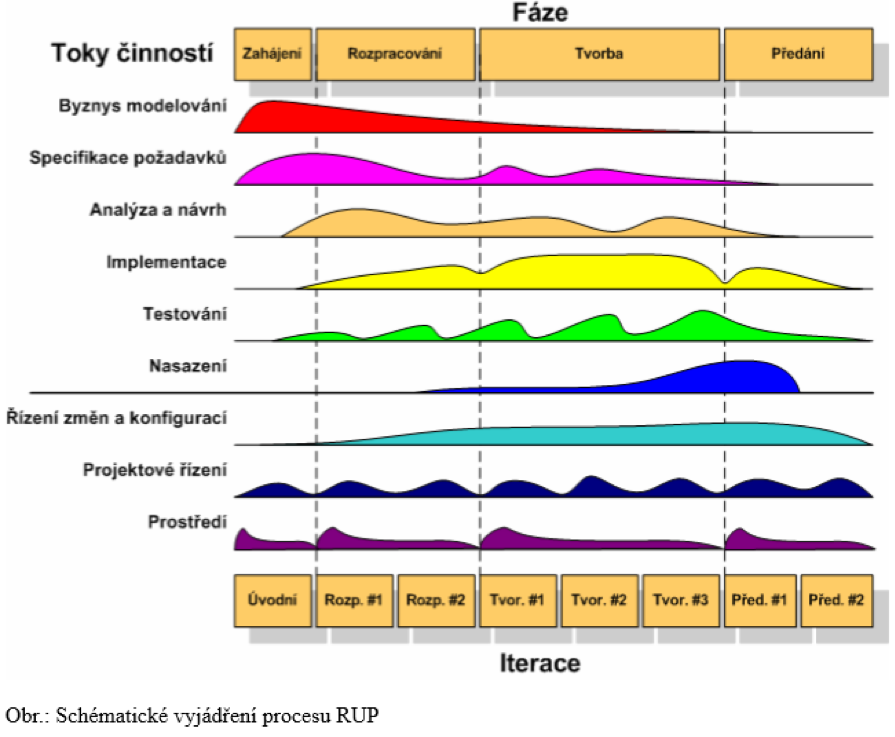
\includegraphics[width=0.65\textwidth]{assets/rup.png}
\end{figure}

V čem se tento přístup liší o dříve zmíněného vodopádového modelu?  Základní rozdíl spočívá v tom, že \textbf{toky činností probíhají souběžně}, i když z obrázku jasně vyplývá, že objem prací se liší podle fáze rozpracování softwarového systému.  Zřejmě, těžiště činností spjatých s byznys modelováním a specifikací požadavků bude v úvodních fázích, zatímco problematika rozmístění softwarových balíků na počítačích propojených sítí (počítačové infrastruktuře) bude záležitostí fází závěrečných.  Celý životní cyklus je pak rozložen do čtyř základních fází (zahájení, rozpracování, tvorba a předání), přičemž pro každou z nich je typická realizace několika iterací umožňující postupné detailnější rozpracování produktu.


\subsubsection{Cykly, fáze, iterace}
Každý \textbf{cyklus vede k vytvoření takové verze systému}, kterou lze \textbf{předat uživatelům a implementuje jimi specifikované požadavky}. Jak již bylo uvedeno v předchozí kapitole, každý takový vývojový cyklus lze rozdělit do \textbf{čtyř} po sobě jdoucích \textbf{fází}: 
\begin{enumerate}
\item \textbf{Zahájení}, kde je původní myšlenka rozpracována do \textbf{vize koncového produktu} a je definován rámec toho, jak celý systém bude vyvíjen a implementován. 
\item \textbf{Rozpracování} je fáze věnovaná \textbf{podrobné specifikaci požadavků} a \textbf{rozpracování architektury} výsledného produktu. 
\item \textbf{Tvorba} je zaměřena na \textbf{kompletní vyhotovení požadovaného díla}.  Výsledné  programové vybavení je vytvořeno kolem navržené kostry (architektury) softwarového systému. 
\item \textbf{Předání} je závěrečnou fází, kdy \textbf{vytvořený produkt je předán do užívání}. Tato fáze zahrnuje i další aktivity jako je beta \textbf{testování}, \textbf{zaškolení} apod. 
\end{enumerate}
Každá fáze může být dále \textbf{rozložena do několika iterací}.

\subsubsection{Iterace}
Iterace je \textbf{úplná vývojová smyčka vedoucí k vytvoření spustitelné verze kódu} reprezentující \textbf{podmnožinu} vyvíjeného cílového produktu, a která je \textbf{postupně rozšiřována každou iterací} až do výsledné podoby. 
\\\\
\noindent\makebox[\textwidth]{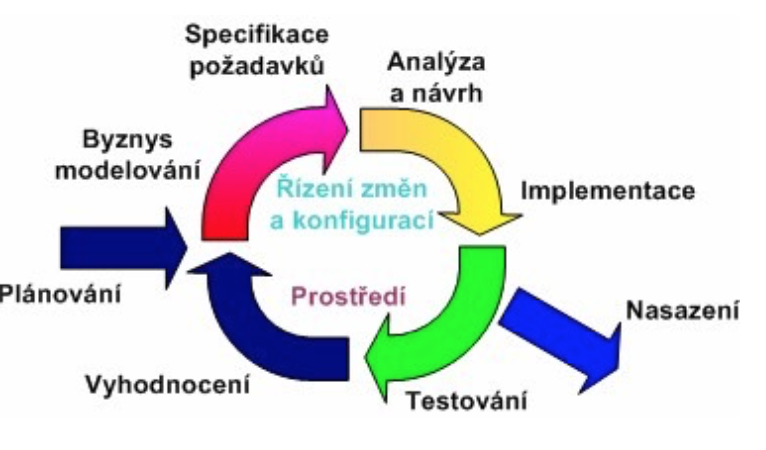
\includegraphics[width=9cm]{assets/swi2}}

\subsubsection{Statická struktura procesu}
Definuje \textbf{KDO} (role), \textbf{CO} (artefaty), \textbf{JAK} (aktivity a jejich toky) a \textbf{KDY} to má vytvořit. Smyslem každého procesu a tedy i softwarového je specifikovat kdo v něm vystupuje, co má vytvořit, jak to má vytvořit a kdy to má vytvořit.  Z tohoto pohledu hovoříme o následujících elementech tvořích strukturu každého softwarového procesu: 
\begin{itemize}
	\item \textbf{Role (pracovníci)} definují chování, kompetence a zodpovědnosti jednotlivých osob (analytik, programátor, projektový manažer apod.) nebo skupiny osob spolupracujících v týmech.  Jednotlivé osoby (lidské zdroje) jsou mapovány na požadované role dle toho, jak jsou požadované kompetence slučitelné se schopnostmi těchto osob.
\item \textbf{Artefakty} reprezentují entity, které jsou v procesu vytvářeny, modifikovány nebo zužitkovány (modely, dokumentace, zdrojové kódy apod.).  Základním artefaktem, který je nosným pro vývoj softwarového systému je \textbf{model} - \textbf{zjednodušení reality umožňující lépe pochopit vyvíjený systém}.
\item \textbf{Aktivity (činnosti)} prováděné pracovníky s cílem vytvořit nebo upravit artefakty (kompilace zdrojových kódů, vytvoření návrhu apod.).
\item \textbf{Toky činností (workflow)} reprezentují posloupnosti aktivit vytvářející požadované produkty (byznys modelování, specifikace požadavků apod.).
\end{itemize}

\subsubsection{Základní a podpůrné toky čínností}
Vývoj softwarového systému je dán celou řadou aktivit a činností, které jsou uspořádány do toků charakteristických svým účelem.  Z tohoto pohledu můžeme hovořit o tzv. základních tocích, jejichž výsledkem je část softwarového produktu (artefakt) a o tocích podpůrných, které nevytváří hodnotu, ale jsou nutné pro realizaci základních toků. 
Základní toky vytvářející vlastní softwarový produkt jsou následující: 
\begin{itemize}
\item \textbf{Byznys modelování} popisuje strukturu a dynamiku podniku či organizace.
\item \textbf{Specifikace požadavků} definuje prostřednictvím specifikace případů použití softwarového systému jeho funkcionalitu.
\item \textbf{Analýza a návrh} zaměřené na specifikaci architektury softwarového produktu.
\item \textbf{Implementace} reprezentuje vlastní tvorbu softwaru, testování komponent a jejich integraci.
\item \textbf{Testování} zaměřené na činnosti spjaté s ověřením správnosti řešení softwaru v celé jeho složitosti.
\item \textbf{Rozmístění} se zabývá problematikou \textbf{konfigurace} výsledného produktu na cílové počítačové infrastruktuře. 
\end{itemize}

\begin{figure}[H]
	\centering
	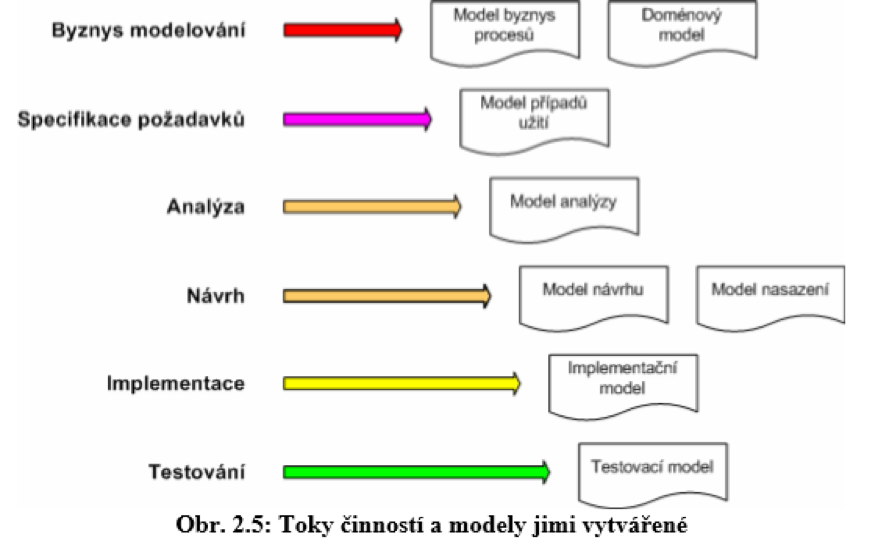
\includegraphics[width=0.65\textwidth]{assets/toky_cinnosti.png}
\end{figure}

\noindent\textbf{Podpůrné toky}, samozřejmě ty nejdůležitější a spjaté s vlastním vývojem, jsou:
\begin{itemize}
\item \textbf{Řízení změn a konfigurací} se zabývá problematikou správy jednotlivých verzí vytvářených artefaktů odrážejících vývoj změn požadavků kladených na softwarový systém.
\item \textbf{Projektové řízení} zahrnující problematiku koordinace pracovníků, zajištění a dodržení rozpočtu, aktivity plánování a kontroly dosažených výsledků.  Nedílnou součástí je tzv. \textbf{řízení rizik}, tedy identifikace problematických situací a jejich řešení.
\item \textbf{Prostředí} a jeho správa je tok činností poskytují vývojové organizaci metodiku, nástroje a infrastrukturu podporující vývojový tým.
\end{itemize}

\subsection{Úrovně vyspělosti}
Úroveň definice a využití softwarového procesu je hodnocena dle stupnice \textbf{SEI (Software Engineering Institute)} \textbf{1 - 5} vyjadřující vyspělost firmy či organizace z daného hlediska. Tento model hodnocení vyspělosti a schopností dodavatele softwarového produktu se nazývá \textbf{CMM (Capability Maturity Model)} a jeho jednotlivé úrovně lze stručně charakterizovat asi takto:

\begin{enumerate}
	\item \textbf{Počáteční (Initial)} -- firma \textbf{nemá definován softwarový proces} a každý projekt je řešen \textbf{případ od případu} (ad hoc).
	\item \textbf{Opakovatelná (Repeatable)} -- firma identifikovala v jednotlivých projektech \textbf{opakovatelné postupy} a tyto je schopna reprodukovat v každém novém projektu.
	\item \textbf{Definovaná (Defined)} -- softwarový proces je \textbf{definován (a dokumentován)} na základě integrace dříve identifikovaných opakovatelných kroků.
	\item \textbf{Řízená (Managed)} -- na základě definovaného softwarového procesu je firma schopna jeho \textbf{řízení} a \textbf{monitorování}.
	\item \textbf{Optimalizovaná (Optimized)} -- zpětnovazební informace získaná \textbf{dlouhodobým procesem monitorování} softwarového procesu je využita ve prospěch jeho optimalizace.
\end{enumerate}

